\documentclass[10pt]{beamer}

\usepackage{polyglossia}
\usepackage{csquotes}
\usepackage{datetime}
\usepackage{fontspec}
\usepackage{microtype}
\usepackage{color}
\usepackage{url}
\usepackage{hyperref}
\usepackage{amsfonts}
\usepackage{amsmath}
\usepackage{amsthm}
\usepackage{subcaption}
\usepackage[backend=biber,style=iso-authoryear,sortlocale=en_US,autolang=other,bibencoding=UTF8]{biblatex}
\usepackage{booktabs}
\usepackage{graphics}
\usepackage{pifont}
\usepackage{ulem}
\usepackage{tikz}

\addbibresource{zotero.bib}

\setdefaultlanguage{english}
\setmainfont{TeX Gyre Termes}
\usetheme{Boadilla}
\usecolortheme{crane}
\setbeamertemplate{title page}[default][rounded=true,shadow=false]
\setbeamertemplate{section in toc}[ball unnumbered]
\setbeamertemplate{bibliography item}{}

\hypersetup{
	pdfencoding=auto,
	unicode=true,
	citecolor=green,
	filecolor=blue,
	linkcolor=red,
	urlcolor=blue
}

\makeatletter
\newcommand*{\currentSection}{\@currentlabelname}
\makeatother

\newcommand{\mathmat}{\ensuremath{\mathbf}}

\title[Graph coarsening \& quality]
{
	Adaptive graph coarsening in the context of local graph quality
}

\newdate{presentation}{16}{09}{2022}
\date[September 2022]{Graph Quality 2022, \displaydate{presentation}}

\author[Marek Dědič]
{
	\underline{Marek~Dědič}\inst{1}\inst{2},
	Lukáš~Bajer\inst{2},
	Jakub~Repický\inst{2},
	Pavel~Procházka\inst{2},
	Martin~Holeňa\inst{3}
}

\institute[CTU \& Cisco]
{
	\inst{1} Czech Technical University in Prague \and
	\inst{2} Cisco Systems, Inc. \and
	\inst{3} Institute of Computer Science, Czech Academy of Sciences
}

% Title card
\AtBeginSection[]{
	\begin{frame}
		\vfill
		\centering
		\begin{beamercolorbox}[sep = 8pt,center,shadow = true,rounded = true]{title}
			\usebeamerfont{title}\insertsectionhead\par%
		\end{beamercolorbox}
		\vfill
	\end{frame}
}

%\AtBeginSection[]{
	%\begin{frame}{\currentSection}
		%\tableofcontents[currentsection]
	%\end{frame}
%}

\begin{document}

\begin{frame}
	\titlepage
	\hfill\usebeamerfont{date}\url{marek@dedic.eu}\hspace{1cm}
	\vspace{0.5cm}
\end{frame}

\section{Problem introduction}

\begin{frame}{Problem introduction}
	\begin{itemize}
		\item Graph algorithms on big graphs -- computationally costly and sometimes even unfeasible.
		\item Our interest: Behaviour of graph algorithms when the graph is coarsened
		\item How much can a graph be coarsened?
		\item Sometimes compressed data \( \implies \) better performace
	\end{itemize}
\end{frame}

\section{Prior art - the HARP method}

\begin{frame}{HARP - learning on coarser graphs}
	\begin{itemize}
		\item HARP - a method for pretraining on simplified graphs
		\item Simplified graphs generated in the way depicted bellow
		\item Embedding trained from the coarsest to the finest graph
	\end{itemize}
	\begin{figure}
		\centering
		\begin{subfigure}[t]{0.38\textwidth}
			\centering
			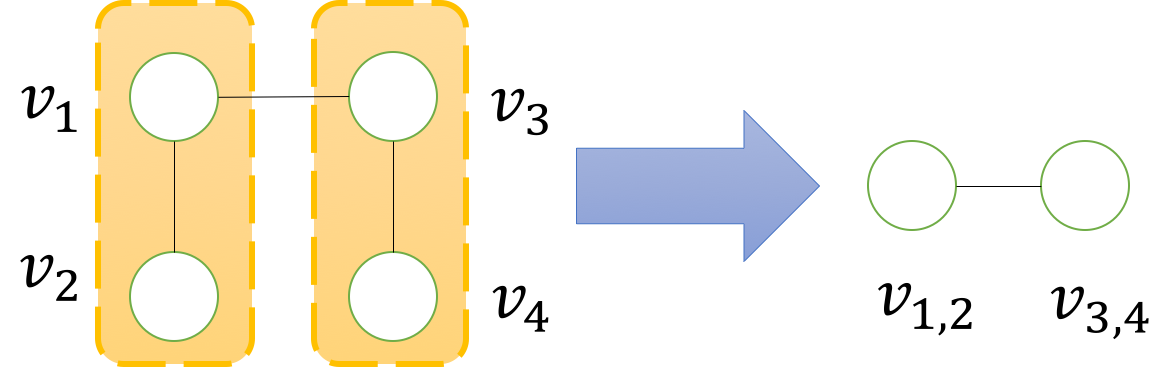
\includegraphics[width=\textwidth]{images/edge_collapsing.png}
			\caption{Edge collapsing}
		\end{subfigure}
		\hspace{2em}
		\begin{subfigure}[t]{0.38\textwidth}
			\centering
			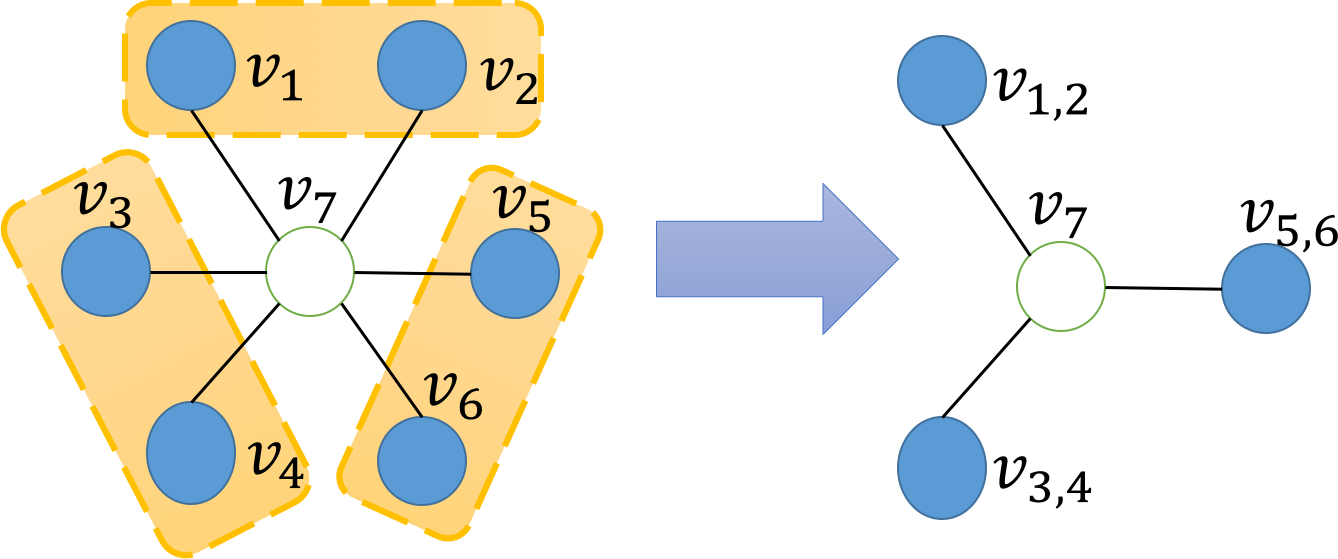
\includegraphics[width=\textwidth]{images/star_collapsing.png}
			\caption{Star collapsing}
		\end{subfigure}
		\caption{HARP coarsening algorithm. \footnote{Images from \cite{chen_harp_2018}.}}
	\end{figure}
\end{frame}

\begin{frame}{HARP pipeline overview}
	\begin{figure}
		\centering
		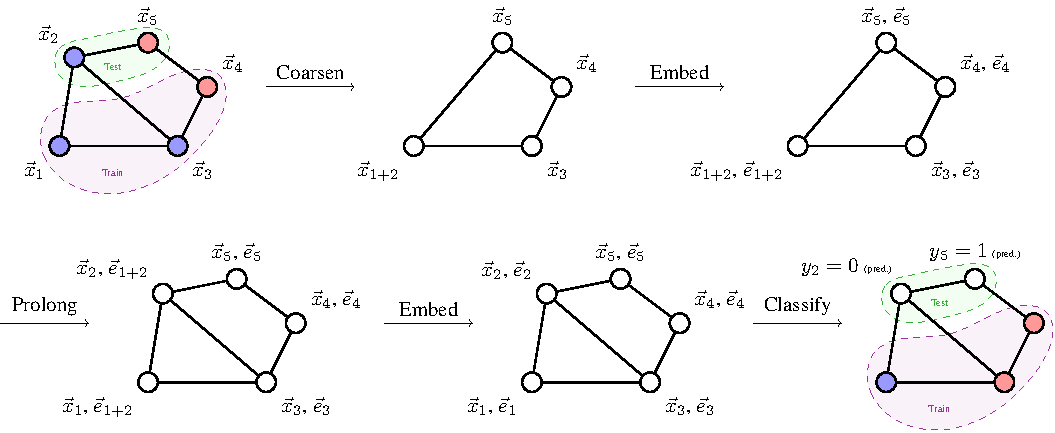
\includegraphics[width=\textwidth]{images/harp-overview/harp-overview.pdf}
	\end{figure}
\end{frame}

\section{Adaptive prolongation}

\begin{frame}{HARP pipeline overview}
	\begin{figure}
		\centering
		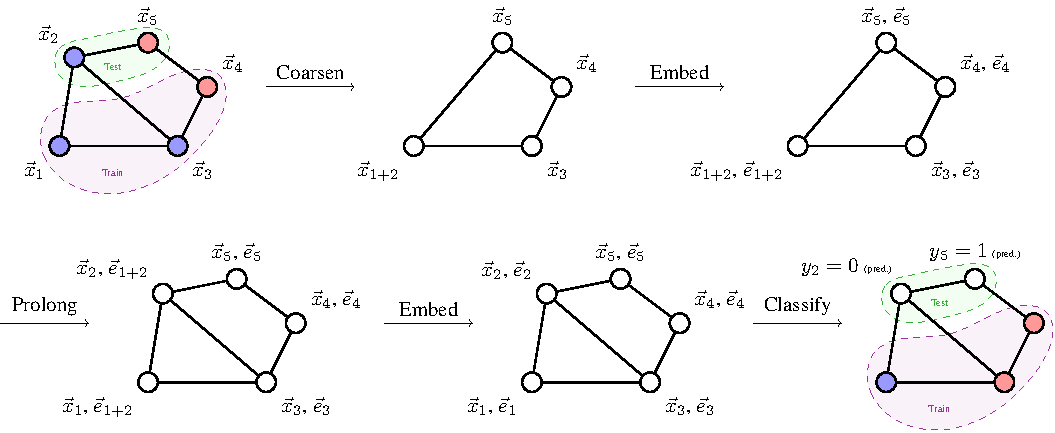
\includegraphics[width=\textwidth]{images/harp-overview/harp-overview.pdf}
	\end{figure}
\end{frame}

\begin{frame}{Deep HARP}
	\begin{figure}
		\centering
		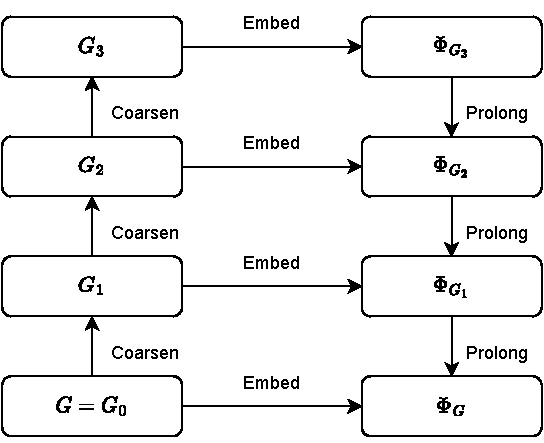
\includegraphics[width=0.6\textwidth]{images/deep-harp/deep-harp.pdf}
	\end{figure}
\end{frame}

\begin{frame}{Adaptive prolongation}
	\begin{itemize}
		\item Graph prolongation (de-coarsening) micro-stepping
		\item Guiding the prolongation based on local properties
		\item Possibly results in different \enquote{model resolution} in different parts of the graph
	\end{itemize}
\end{frame}

\begin{frame}{Adaptive prolongation}
	\begin{figure}
		\centering
		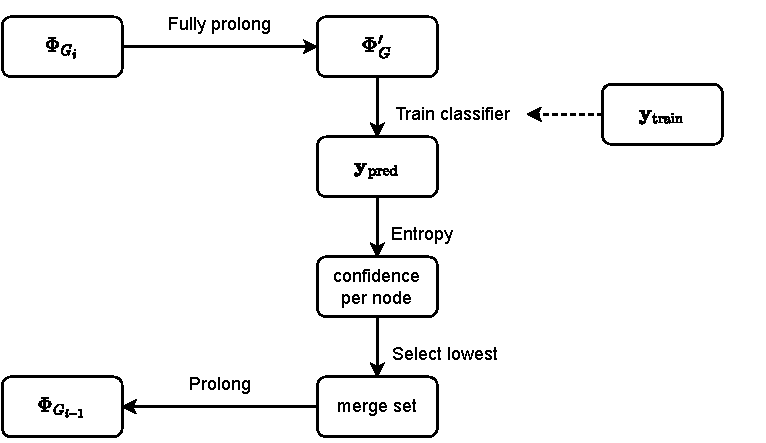
\includegraphics[width=0.8\textwidth]{images/adaptive-prolongation/adaptive-prolongation.pdf}
	\end{figure}
\end{frame}

\begin{frame}{Adaptive prolongation - experimental verification}
	\begin{figure}
		\centering
		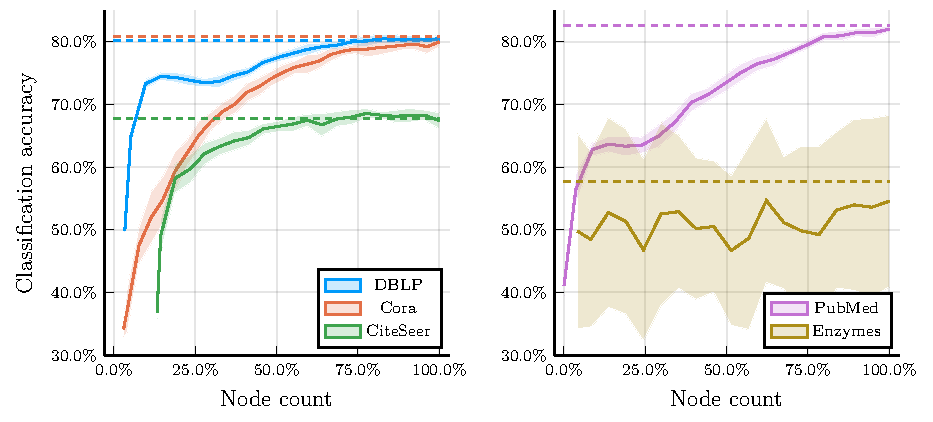
\includegraphics[width=\textwidth]{images/adaptive-coarsening/adaptive-coarsening.pdf}
		\caption{Prediction accuracy with guided prolongation.}
	\end{figure}
\end{frame}

\section{Alternative approaches to coarsening}

\begin{frame}{HARP coarsening}
	\begin{figure}
		\centering
		\begin{subfigure}[t]{0.38\textwidth}
			\centering
			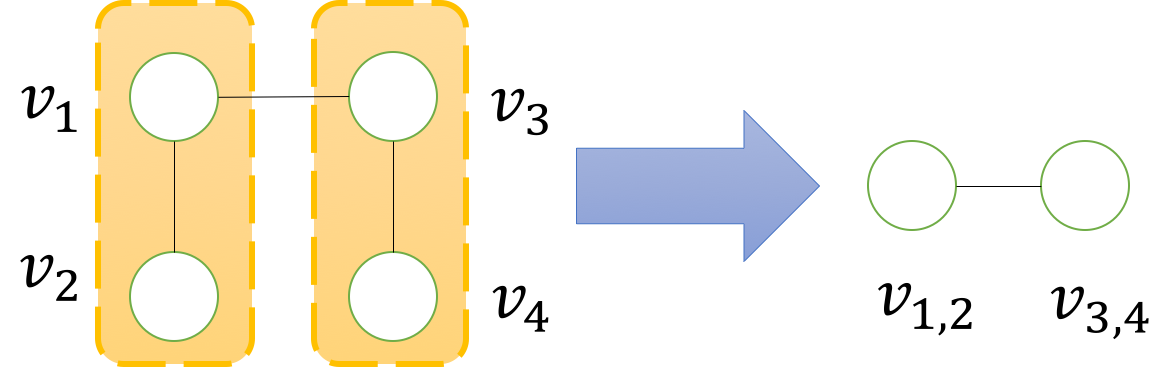
\includegraphics[width=\textwidth]{images/edge_collapsing.png}
			\caption{Edge collapsing}
		\end{subfigure}
		\hspace{2em}
		\begin{subfigure}[t]{0.38\textwidth}
			\centering
			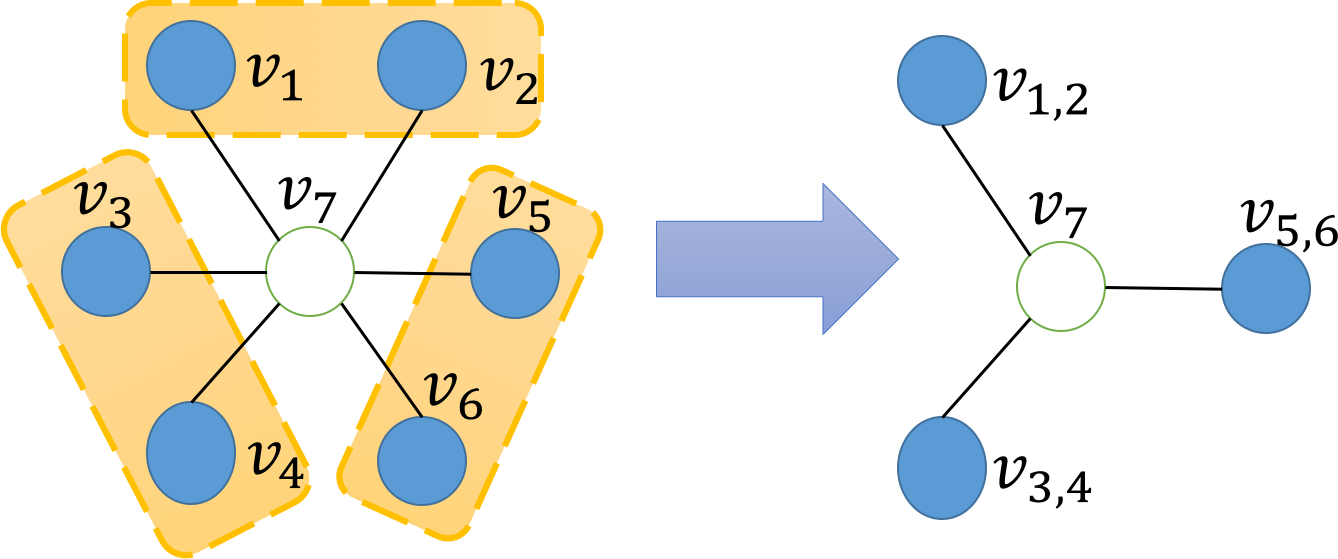
\includegraphics[width=\textwidth]{images/star_collapsing.png}
			\caption{Star collapsing}
		\end{subfigure}
		\caption{HARP coarsening algorithm. \footnote{Images from \cite{chen_harp_2018}.}}
	\end{figure}
\end{frame}

\begin{frame}{Evaluated approaches to coarsening}
	\begin{itemize}
		\item Original HARP
		\item Coarsening based on the personalized PageRank algorithm
		\item Coarsening based on heat diffusion
		\item Evolutionary optimization of coarsening
	\end{itemize}
\end{frame}

\begin{frame}{Experimental comparison of coarsening approaches}
	\begin{figure}
		\centering
		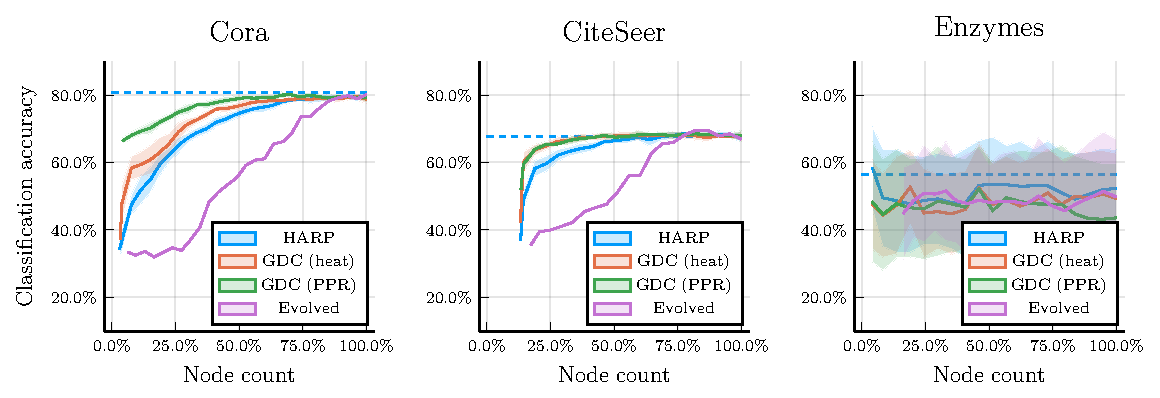
\includegraphics[width=\textwidth]{images/coarsening-algorithms/coarsening-algorithms.pdf}
		\caption{Prediction accuracy with different algorithms.}
	\end{figure}
\end{frame}

\section{Conclusion}

\begin{frame}{Conclusion}
	\centering
	\begin{itemize}
		\item Studying GNN behaviour while coarsening a graph
		\item A new re-formalization of HARP, allowing for a more general approach to graph coarsening
		\item 3 new coarsening strategies
		\item Hopefully a paper in sight
	\end{itemize}
\end{frame}

\begin{frame}
	\titlepage
	\hfill\usebeamerfont{date}\url{marek@dedic.eu}\hspace{1cm}
	\vspace{0.5cm}
\end{frame}

\end{document}
